\documentclass[a4paper]{article}

\usepackage[dutch]{babel}
\usepackage{geometry}
\usepackage[utf8]{inputenc}
\usepackage{hyperref}
\usepackage{graphicx}

% dimensions
\geometry{left=3cm, top=3cm, right=3cm, bottom=3cm}

% font
\usepackage{DejaVuSans}
\renewcommand*\familydefault{\sfdefault}
\usepackage[T1]{fontenc}

% image
\graphicspath{ {img/} }

% lists
\providecommand{\tightlist}{%
\setlength{\itemsep}{0pt}\setlength{\parskip}{0pt}}

% preamble
\title{User Manual}
\author{Tim Visée \& Nathan Bakhuijzen}
\date{October 2018}

\begin{document}

  \pagenumbering{gobble}
  \maketitle
  \begin{figure}[h]
    \centering
    
\includegraphics[width=\linewidth]{cant-touch-this}
  \end{figure}
  \clearpage

  \section{Goal}
  The purpose of this manual is twofold:
  \begin{itemize}
    \tightlist
    \item To inform research how to use the platform to execute experiments and
      conduct research
    \item To inform future developers how to continue developing the platform
  \end{itemize}

  \section{Problem Definition}
  \textit{What physical motions are natural, effortless and easy, in order to
    control a computer or other digital device?}

  Questions of this nature can be answered using the \textit{Can't Touch This}
  platform. \textit{Can't Touch This} aims to be a platform for researchers that
  would like to conduct research in the field of touchless computer systems. We
  believe that our platform allows researchers to build a strong foundation for
  the future of touchless control. Giving researchers the opportunity to conduct
  research improves the chance for touchless control of computers only seen in
  futuristic movies and tv shows.

  \subsection{Motivation}
  At the start of the KB-80 minor, students were given a choice in the subject
  of the research. Mister Hani introduced us to a series of subjects, of which
  the LeapMotion project was the most interesting to us. The idea of the
  LeapMotion was to create or extend existing software to enable people to
  control a computer without touching any peripherals, like keyboards and mice.

  \subsection{Background information}
  Research in the field of touchless computer systems is motivated by the desire
  for these systems in sterile environments. For example, surgeons often make
  use of computer systems to aid them during their surgeries by providing
  crucial information such as CT, MRI and X-ray scans. This is where touchless
  computer systems come in. These systems allows surgeons on control a computer
  without the need for physical peripherals.
  \clearpage

  \section{Installation Guide}
  % •	Platform and OS version
  \subsection{Requirements}
  \begin{itemize}
    \tightlist
    \item A computer with the Windows (7+), OSX (10.7+, Lion+) or
      Linux (kernel 2.6.18+) operating system
    \item An installation of the LeapMotion
      \href{https://developer.leapmotion.com/sdk/v2}{SDK}
    \item An installation of the
      \href{https://rust-lang.org}{Rust} programming language
    \item The physical LeapMotion device itself
  \end{itemize}

  % •	Other software dependencies
  \subsection{Software Dependencies}
  The \textit{Can't Touch This} platform is written using the
  \href{https://rust-lang.org}{Rust programming language}. This means that the
  operating system that the platform will run on must support the Rust language.
  Fortunately, Rust runs on all popular operating systems today, shown above in
  the list of requirements. An up-to-date list of all supported versions can be
  found on the
  \href{https://forge.rust-lang.org/platform-support.html}{Rust website}.
  Additonally, the \textit{Can't Touch This} platform requires the LeapMotion
  \href{https://developer.leapmotion.com/sdk/v2}{SDK} to provide all necessary
  sensor data. Just like the Rust programming language, the LeapMotion SDK can
  be installed on all platforms.

  % •	External resources needed to run the prototype.
  \subsection{External resources}
  To be written.

  % •	External resources (or tools) needed to continue developing the prototype
  \subsection{External development tools}
  To be written.
  \clearpage

  % 2. User instructions
  % Step by step instructions on how to use the research platform to conduct research.
  % Checklist:
  %   •	Instructions to run the experiment (explained in build plan)
  %   •	Aimed at non technical researchers
  %   •	Include screenshots when possible

  % Bonus points: make a video of the instructions, upload to youtube and include link in manual
  % Note: even if video instructions are created the manual should still have written instructions


  % 3. Requirements
  % Here you describe what requirements you have already gathered from the client.
  % Checklist:
  %   •	What requirements are done
  %   •	What requirements are still open
  %   •	Prioritizing of requirements (MOSCOW)


  % 4. Software Architecture Diagram
  % 4.1 Context view
  % Describe the relationships, dependencies, and interactions between the system and its environment (the people, system.. and external entities with which it interacts). Your system in this view is represented by a blackbox interacting with external entities. See example in Figure 1.
  % 4.2 Functional view
  % Describe the system’s runtime functional elements and their responsibility, interfaces and primary int

  % Figure 1. Example of a context view

  % methodology:
  %   •	Represent each subcomponent of the system with a box in the figure. 
  %   •	Link the system subcomponents with connectors. These connectors define the interaction between the elements that use it. 
  %   •	Under the figure explain each subcomponent, and give:
  %   •	Inputs
  %   •	Outputs
  %   •	What functionality is available
  %   •	How to invoke each functionality (commands, syntax, …etc).
  \section{Architecture Diagrams}
  \begin{figure}[h]
    \caption{Context Diagram}
    \centering
    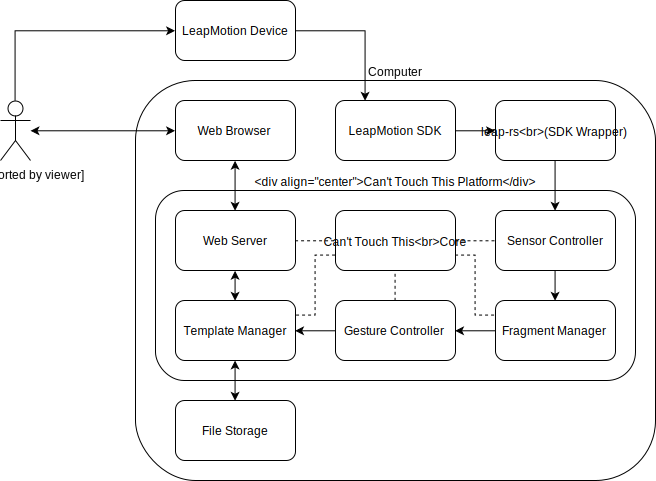
\includegraphics[width=\linewidth]{context-diagram}
  \end{figure}
  \begin{figure}[h]
    \caption{Context Diagram}
    \centering
    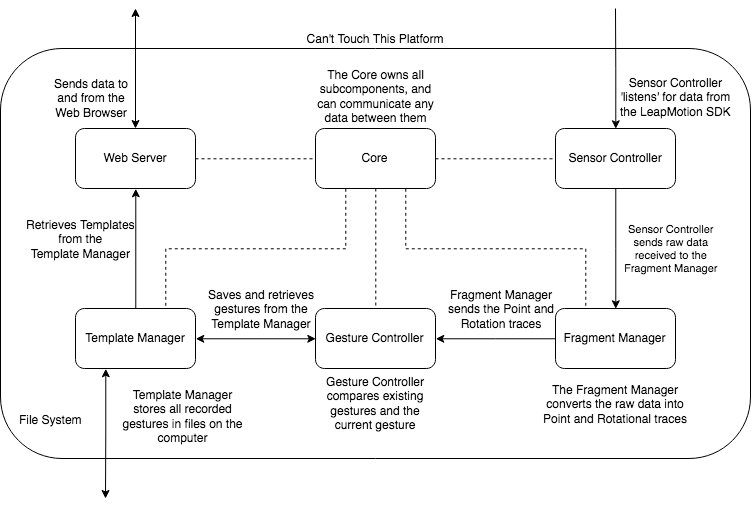
\includegraphics[width=\linewidth]{functional-diagram}
  \end{figure}
  \clearpage

  % 5. Domain model
  % In the domain model you list all:
  %   •	API interfaces
  %   •	Subsystems

  % 6. Test report
  % Add this section even if you did not do any formal testing on the system. 
  % Checklist:
  %   •	What is the quality of the code
  %   •	What has already been tested
  %   •	What are the known bugs in the system

  % known issues
  \section{Known Issues}
  \begin{itemize}
    \tightlist
    \item \textit{Can't Touch This} may crash upon running the release version
      of the exectable
    \item On macOS, the LeapMotion device may never give data to begin with
    \item On macOS, the LeapMotion device may stop recording data randomly
    \item On macOS, the application may not run well when minimalizing the
      backend application
  \end{itemize}
\end{document}
